\section{Neural Networks}
Artificial neural networks (ANNs) represent a class of machine learning (ML) algorithms that simulate the learning mechanism observed in the human brain \cite{aggarwal2018neural}. 

The fundamental building blocks of the human nervous system are called \textit{neurons}. 

\subsection{Biological neurons}

Neurons are a specialized type of cells found in the human body, responsible for transmitting nerve impulses.

As shown in \Fig~\ref{fig:neurons}, neurons establish connections with each other through \textit{axons} and \textit{dendrites}, and the regions where these connections occur are known as \textit{synapses}. This enables communication between neurons through electrical events, known as \textit{action potentials}, which occur at the synapses \cite{APS}. 

Each neuron receives stimuli from multiple neurons simultaneously, and these inputs are summed. Action potentials are generated only when the summed value crosses a specific \textbf{threshold}, at which point the neuron emits a \textit{spike}. An example of the \textit{spiking} mechanism is illustrated in \Fig~\ref{fig:spking}.

\begin{figure}[h]
	\centering
	\begin{subfigure}{.5\textwidth}
		\centering
		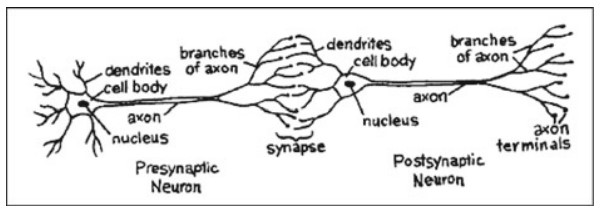
\includegraphics[width=0.7\linewidth]{ImageFiles/NeuralNetworks/neuron}
		\caption{Human neurons}
		\label{fig:neurons}
	\end{subfigure}%
	\begin{subfigure}{.5\textwidth}
		\centering
		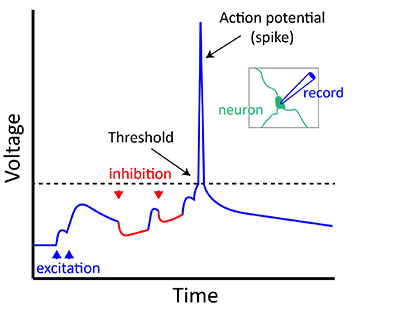
\includegraphics[width=0.5\linewidth]{ImageFiles/NeuralNetworks/spiking}
		\caption{Neuron spike after reaching the threshold}
		\label{fig:spking}
	\end{subfigure}
	\caption{Mechanisms in the human neuron}
\end{figure}

Furthermore, the strengths of synaptic connections frequently undergo changes in response to external stimuli \cite{aggarwal2018neural}. While the precise mechanisms of information processing in the brain are still unknown, the propagation of action potentials across vast networks of fired neurons is believed to lead to the brain \textbf{learning} and \textbf{thinking} process.

\subsection{Artificial neurons}

ANNs aim to simulate the biological mechanisms of the brain by utilizing \textit{artificial} neurons as their fundamental building blocks. These artificial neurons are responsible for performing basic computations within the network. To simplify the terminology, the term "neurons" will denote artificial neurons.
An illustration of the functioning of these neurons is presented in \Fig~\ref{fig:art_neuron}. The neurons are interconnected through weights, which simulate the role of synapses. A higher weight value indicates a stronger connection.

\begin{figure}[h]
	\centering
	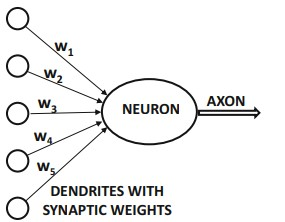
\includegraphics[width=0.4\linewidth]{ImageFiles/NeuralNetworks/art_neuron}
	\caption{Artificial neuron}
	\label{fig:art_neuron}
\end{figure}

Consequently, each neuron receives inputs from other neurons, which are then weighted and summed together. Additionally, a possible bias can be added to the summed inputs. The resulting value is then passed through an \textit{activation function} $\sigma$, mimicking the spiking mechanism observed in the human brain and determining the neuron output.

\[
	\sigma (z) = \sigma (b + \sum w_i \cdot x_i)
\]

The neuron model is commonly referred to as the \textit{Perceptron}. The first perceptron model utilized a simple step function as the activation.

The complete sequence of operations is shown in \Fig~\ref{fig:percep_full} where the activation is a simple \textit{step function}.

\begin{figure}[h]
	\centering
	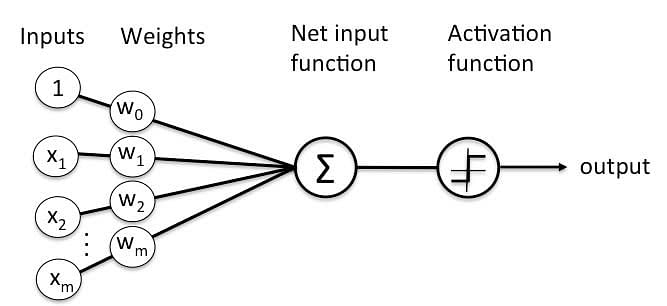
\includegraphics[width=0.5\linewidth]{ImageFiles/NeuralNetworks/percep_full}
	\caption{Sequence of operations in an artificial neuron \cite{WPBGP}}
	\label{fig:percep_full}
\end{figure}

\subsection{Activation functions}

The activation function (AF) plays a crucial role in determining the activation level of a node. In the early perceptron model, the step function was commonly used as the AF, producing binary outputs. However, for complex problems, this binary nature is often insufficient. It has been discovered that not all AFs are equally effective and must be chosen carefully.
The true power of ANNs emerges from the composition of specific types of AFs, which enables the network to enhance its expressiveness and tackle more complex tasks \cite{aggarwal2018neural}. Nowadays, ANNs employ various AFs, typically non-linear, to model complex data. Here are some of the most common activation functions.

\vspace{0.2cm}
\textbf{Sigmoid}

The sigmoid function maps the input to a smooth S-shaped curve, producing outputs between 0 and 1. It is suitable for binary classification problems and can be used in the output layer of a neural network. However, it is important to note that the sigmoid function suffers from the issue of gradient vanishing, making it less suitable for deep neural networks. In \Fig~\ref{fig:sigmoid} is shown a plot of the sigmoid function.

\vspace{0.2cm}
\textbf{Rectified Linear Unit}

The Rectified Linear Unit (ReLU), shown in \Fig~\ref{fig:relu} sets the output to zero for negative inputs and maintains a linear relationship for positive inputs. It is widely used in hidden layers of deep neural networks due to its simplicity and ability to mitigate the vanishing gradient problem. The ReLU function will be widely used in this case study.

\vspace{0.2cm}
\textbf{Hyperbolic Tangent Function}

As shown in \Fig~\ref{fig:tanh}, the Hyperbolic Tangent (tanh) function is similar to the sigmoid, the tanh function also maps inputs to a range between -1 and 1. It provides stronger gradients than the sigmoid function.

\vspace{0.2cm}
\textbf{Softmax Function}

The softmax function is frequently employed in the output layer of an ANN for multiclass classification problems. It normalizes the outputs to form a probability distribution, ensuring that the sum of the output values is equal to 1. The softmax function can be seen as an extension of the sigmoid applied to each output neuron, followed by a normalization step.

\begin{figure}[h]
	\centering
	\begin{subfigure}{.33\textwidth}
		\centering
		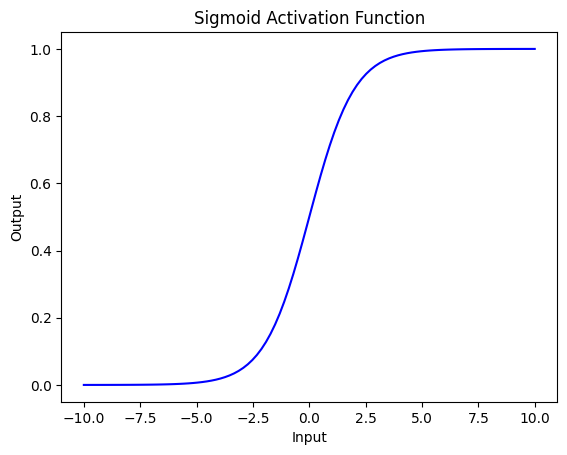
\includegraphics[width=0.8\linewidth]{ImageFiles/NeuralNetworks/sigmoid}
		\caption{Sigmoid function}
		\label{fig:sigmoid}
	\end{subfigure}%
	\begin{subfigure}{.33\textwidth}
		\centering
		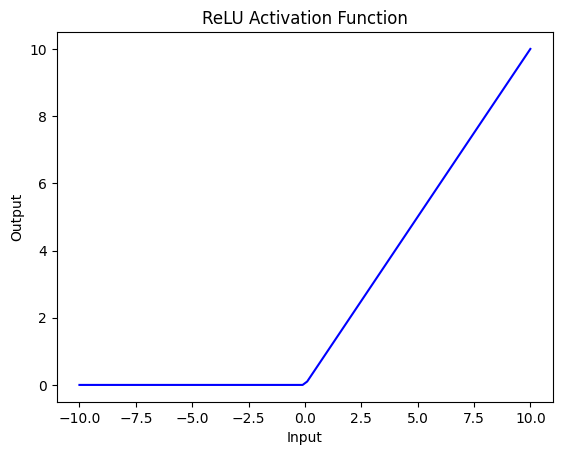
\includegraphics[width=0.8\linewidth]{ImageFiles/NeuralNetworks/relu}
		\caption{ReLU function}
		\label{fig:relu}
	\end{subfigure}%
	\begin{subfigure}{.33\textwidth}
		\centering
		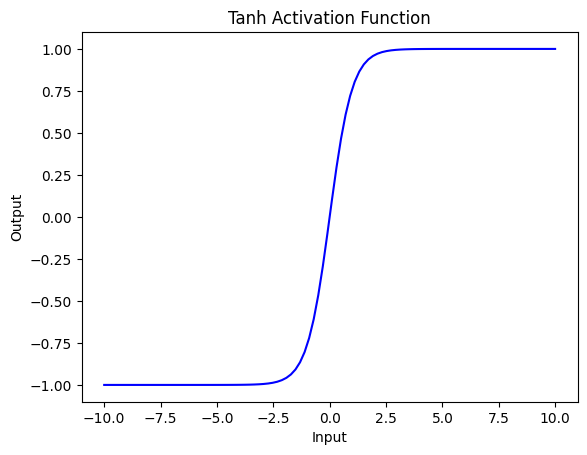
\includegraphics[width=0.8\linewidth]{ImageFiles/NeuralNetworks/tanh}
		\caption{Tanh function}
		\label{fig:tanh}
	\end{subfigure}
	\caption{Activation functions plots}
\end{figure}

\subsection{Layers}

As mentioned earlier, ANNs consist of numerous fundamental computational units known as neurons. These neurons are arranged in \textit{layers} which are interconnected with each other. In an artificial neural network (ANN), there can be multiple layers that can be classified into three main categories:

\begin{itemize}
	\item \textit{Input} layer: The input layer receives the initial data or features that are fed into the network. Each neuron in this layer represents a specific input feature, and there is usually one neuron per input feature.
	
	\item \textit{Hidden} layer(s): They are located between the input and output layers and are responsible for processing and transforming the input data through complex computations. ANNs can have one or more hidden layers, and each layer consists of multiple neurons. These hidden layers enable the network to learn and extract higher-level representations of the input data.
	
	\item \textit{Output} layer: This is the final layer of the network, responsible for producing the desired output or prediction based on the processed information from the hidden layers. The number of neurons in the output layer depends on the type of problem being solved. For example, in binary classification, there is usually one neuron for each class, while in multi-class classification, the number of neurons matches the number of distinct classes.
\end{itemize}

Some networks may have additional types of layers, such as \textit{recurrent} layers for sequential data or \textit{convolutional} layers for image processing. However, the input, hidden, and output layers are the three fundamental classes that are commonly found in most ANNs.

The input and output layers are fundamental components of any ANN. When at least one hidden layer is introduced, the network becomes a \textit{deep} neural network. By increasing the depth, i.e. number of layers, or width, i.e. number of neurons per layer, the network expressiveness can be enhanced, enabling it to model complex data and processes.

Although there are certain guidelines for the selection of network architecture, there is currently no theory able to determine the optimal depth and width of a neural network. The selection process largely relies on experimentation and iterative refinement.

An ANN with a low number of neurons may not be able to properly capture the complexities of the data, resulting in high training error. On the other side, an excessive number of neurons may lead to overfitting, where the network becomes too specialized on the training data, resulting in limited generalization capability on unseen data.

Achieving the right balance between model complexity and generalization capability is a crucial task when designing an ANN architecture. It often involves techniques such as \textit{regularization}, \textit{cross-validation} to mitigate the risk of overfitting and achieve optimal generalization performance.

\subsection{Multilayer perceptron}

One of the most typical \textit{feed-forward} neural networks type is the \textit{multilayer perceptron} (MLP). It is essentially an ANN that includes at least one hidden layer. In the MLP, each neuron in a given layer is fully connected to all the neurons in both the previous and subsequent layers. This connectivity arrangement enables the flow of information in a unidirectional manner, from the input layer through the hidden layers to the output layer.  An example of a MLP with one hidden layer is shown in \Fig~\ref{fig:mlp}.

\begin{figure}[h]
	\centering
	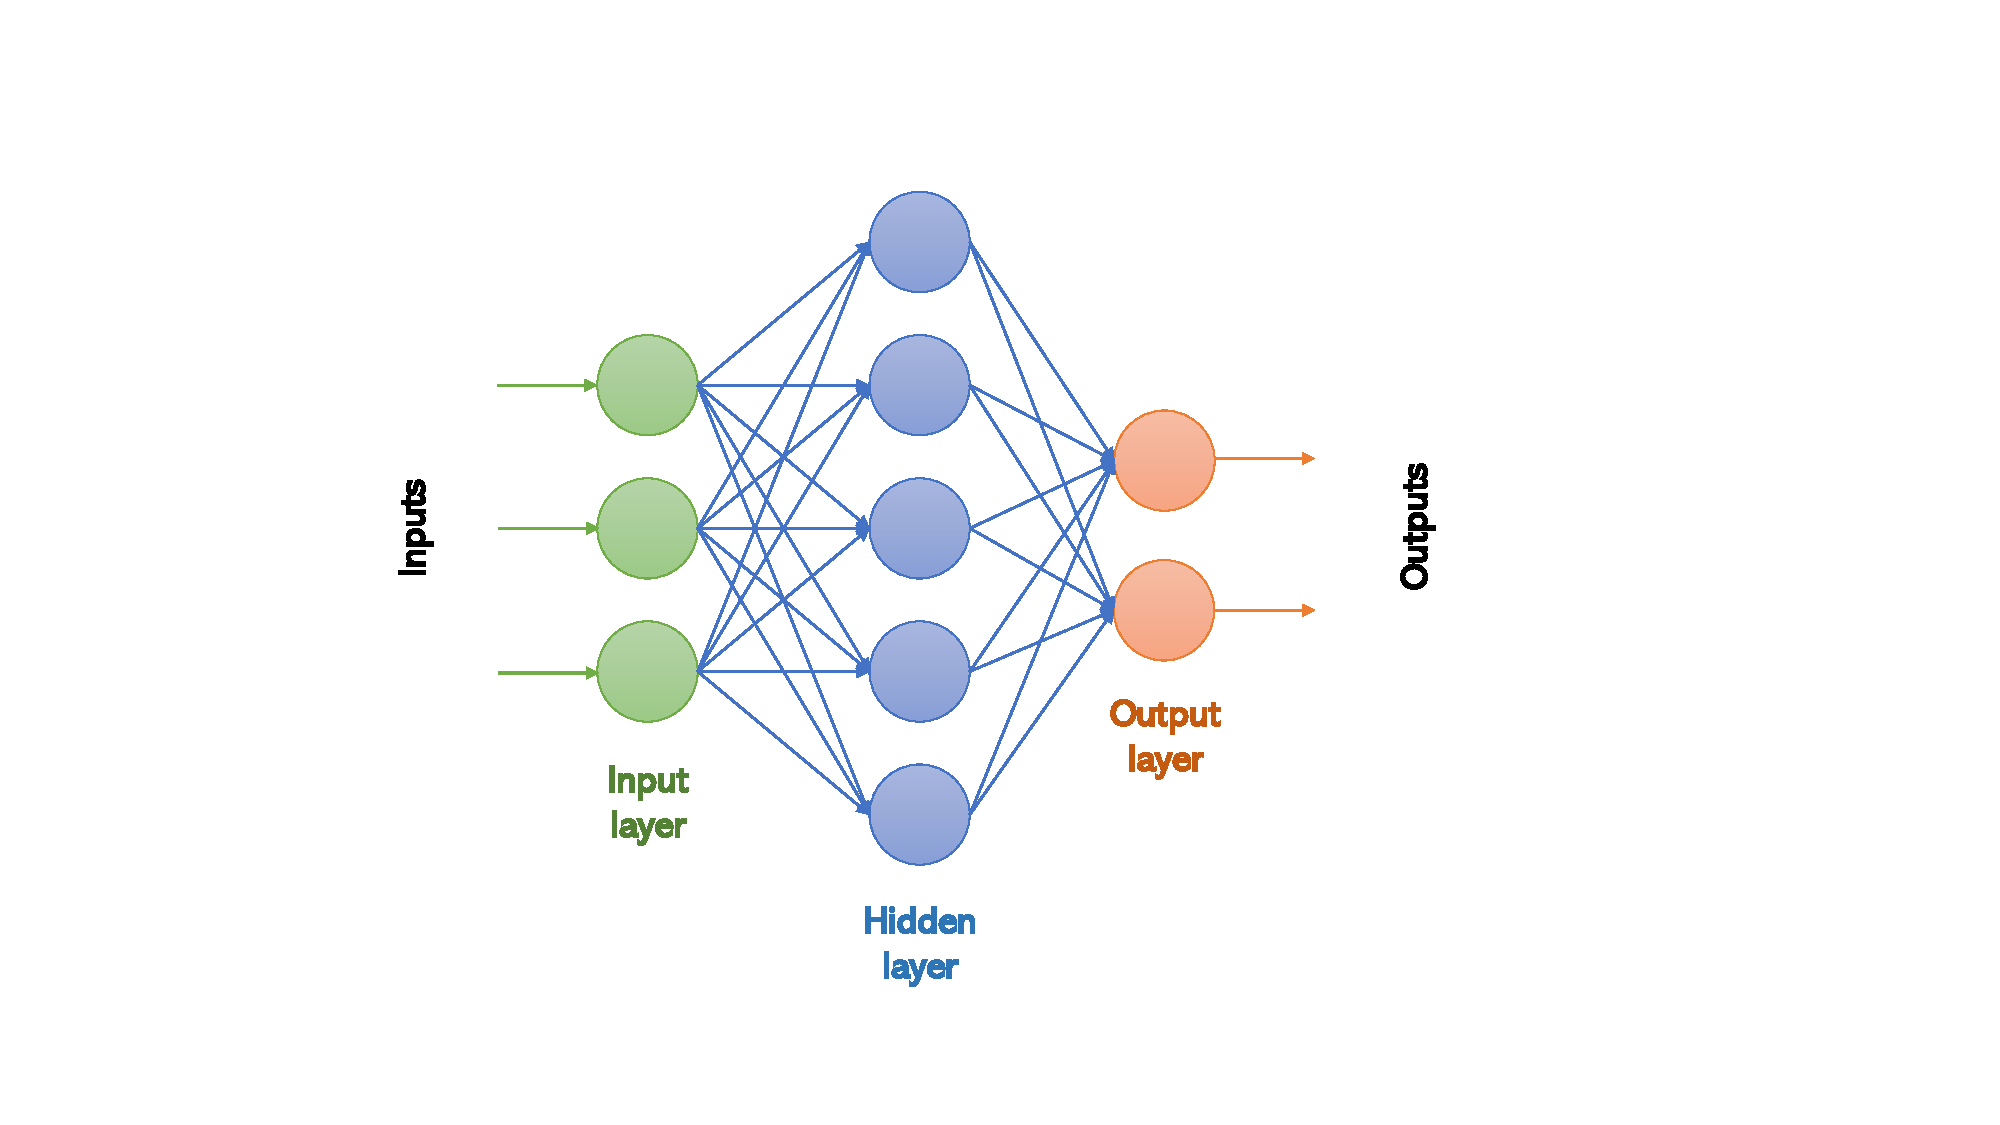
\includegraphics[width=0.9\linewidth]{ImageFiles/NeuralNetworks/mlp}
	\caption{Example of a MLP with one hidden layer}
	\label{fig:mlp}
\end{figure}

However, the MLP suffers from some limitations. One important challenge is the explosion of parameters due to the extensive interconnections between neurons. This can become a problem in architectures with a large number of neurons, leading to computational and memory overheads.

Furthermore, the MLP is not well-suited for tasks involving image processing, particularly when it comes to recognize translations. Its architecture lacks of mechanisms to handle spatial relationships in images effectively.

To overcome these limitations, other types of ANN, such as \textit{convolutional} neural networks (CNNs), have been developed specifically for image processing tasks. CNNs leverage convolutional layers and pooling operations to capture local patterns and spatial relationships, making them more effective in tasks like image recognition and classification.

In this particular case study, an MLP will be utilized due to its simple and comprehensible architecture. While there may be other neural network architectures better suited for certain tasks, the choice of an MLP is driven by the need for simplicity and interpretability. By using an MLP, the focus can be placed on understanding the underlying mechanisms and interpreting the results.

\subsection{Training}

The \textit{learning} process in an ANN is typically achieved by feeding the data to the network, allowing it to automatically adjust its parameters. As a result, there is no need to explicitly define specific behaviors. Depending on the available data, the learning process can be categorized as follows:


\begin{itemize}
	\item \textit{Supervised} Learning: It uses labeled data, where each input is associated with a corresponding target output. The network learns to map inputs to outputs by minimizing the discrepancy between its predicted output and the true target output.
	\item \textit{Unsupervised} Learning: It involves training the network on unlabeled data, without explicit target outputs. The network learns to identify patterns, structures, or representations within the data without any specific guidance.
	\item \textit{Reinforcement} Learning: In case, the network learns through interactions with an environment. It receives feedback in the form of rewards or penalties based on its actions, enabling it to optimize its behavior over time. Therefore, the objective is to acquire the ability to identify and select the best actions to take in order to achieve the best possible outcomes.
\end{itemize}

There are also variations and combinations of these learning processes, such as \textit{semi-supervised} learning, where a limited amount of labeled data is combined with a larger amount of unlabeled data for training. The specific learning process employed depends on the nature of the problem, available data, and desired outcomes.

In this case study, specifically with the utilization of an MLP, the applied learning technique is known as \textit{back-propagation}. It is a supervised learning method that consists of two distinct phases during training:
\begin{enumerate}
	\item \textit{Forward} Propagation: In this phase, the input data is fed into the MLP, and the network processes this data through its layers, producing an output. The prediction is then compared with the desired target, and the difference, known as the \textit{loss} or \textit{error}, is calculated with a proper \textit{loss function};
	\item \textit{Backward} Propagation: The error calculated in the forward propagation phase is propagated backward through the network. The gradients of the error with respect to the network's parameters (weights and biases) are computed. These gradients are then used to adjust the parameters, updating them in a way that minimizes the error.
\end{enumerate}

The two phases described can be illustrated in \Fig~\ref{fig:backprop}. During the forward phase, the neural network computes the predicted output $\hat{y}$ based on the input data. In the backward phase, the network updates its weights by utilizing the gradient of the cost function $J$ with respect to the weights. This gradient provides the necessary information for adjusting the weights in a way that minimizes the cost function and improves the overall performance of the network.

\Fig~\ref{fig:backprop} visually represents these two phases, showcasing the flow of information from the input through the hidden layers to the output layer during the forward phase, and the subsequent backpropagation of the gradients during the backward phase for weight updates.

\begin{figure}[h]
	\centering
	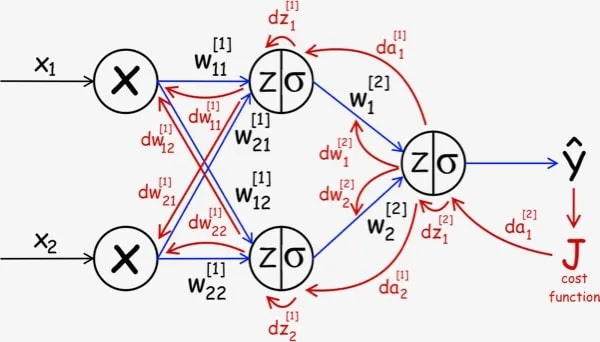
\includegraphics[width=0.5\linewidth]{ImageFiles/NeuralNetworks/backprop}
	\caption{Back-propagation algorithm \cite{UIBASP}}
	\label{fig:backprop}
\end{figure}

By iteratively repeating the forward and backward propagation steps on different input examples, the MLP gradually learns to adjust its parameters to minimize the overall error and improve its performance on the given task. 



During the training process, the \textit{train} set is partitioned into "portions" that are fed into the network. In each iteration, all the portions are processed, and the internal parameters of the network are adjusted. These iterations are commonly referred to as \textit{epochs}. The size of each portion fed into the network is known as the \textit{batch} size.

The utilization of a batch size training serves two key purposes. Firstly, it helps to mitigate the risk of poor generalization capability by exposing the network to a diverse range of examples within each batch. Secondly, it facilitates faster convergence towards good solutions as the network updates its weights based on the average error computed over the batch. However, it is important to note that a small batch size does not guarantee the attainment of global optima, as the network may become trapped in local optima or sub-optimal solutions \cite{KANDEL2020312}.

The choice of an appropriate batch size involves a trade-off between computational efficiency and achieving accurate and generalizable results. Different batch sizes can be experimented with to find the optimal balance for the specific problem at hand.

\subsection{Loss functions}

The loss function quantifies the difference between the network's prediction and the target output. Multiple loss functions are available, and their selection can significantly impact the results obtained. Consequently, choosing an appropriate loss function is a key aspect in designing an ANN since the optimization of network parameters relies on it. In this regard, it is possible to categorize loss functions into two distinct categories \cite{CLFML}:
\begin{enumerate}
	\item \textit{Regression} losses: They are employed when the output is a continuous variable. The most commonly used regression loss functions include the \textit{Mean Squared Error} (MSE) and the \textit{Mean Absolute Error} (MAE);
	\item \textit{Classification} losses: Used when the output is a categorical variable. These loss functions focus on measuring the confidence or certainty of the network's predictions. Two commonly used classification loss functions are the Hinge loss and the Cross Entropy loss (CE).
\end{enumerate}

\subsection{Optimization algorithm}

As previously mentioned, the parameters of the network are updated through the minimization of a loss function. To achieve this, an \textit{optimization} algorithm is employed \cite{Goodfellow-et-al-2016}. In ML, the most popular one is indeed the \textit{gradient descent}, which serves as foundation for many modern optimization algorithms. It has been widely adopted due to its simplicity and effectiveness.

The Gradient Descent algorithm begins by initializing the parameters of the model with initial values. The objective is to update the weights iteratively in order to minimize the loss function. This is achieved by computing the gradient, which represents the direction of steepest descent of the loss function, and then updating the parameters by taking a step in the opposite direction of the gradient.

\[
	w_{ij}^{t+1} = w_{ij}^t - \alpha\frac{\partial J}{\partial w_{ij}}
\]

The \textit{hyperparameter} $\alpha$ is called \textit{learning rate}. It influences how far the algorithm moves in the opposite direction of the gradient. A higher learning rate results in more substantial parameter updates, potentially leading to faster convergence. However, a very high learning rate can lead to instability or overshooting of the optimal solution. Conversely, a lower learning rate corresponds to smaller steps, ensuring more cautious and gradual updates. This can enhance stability, but it may also slow down the convergence process.

In \Fig~\ref{fig:graddesc}, a graphical representation is provided to illustrate the functioning of the gradient descent algorithm when applied to a problem involving a single parameter and a quadratic cost function.

\begin{figure}[h]
	\centering
	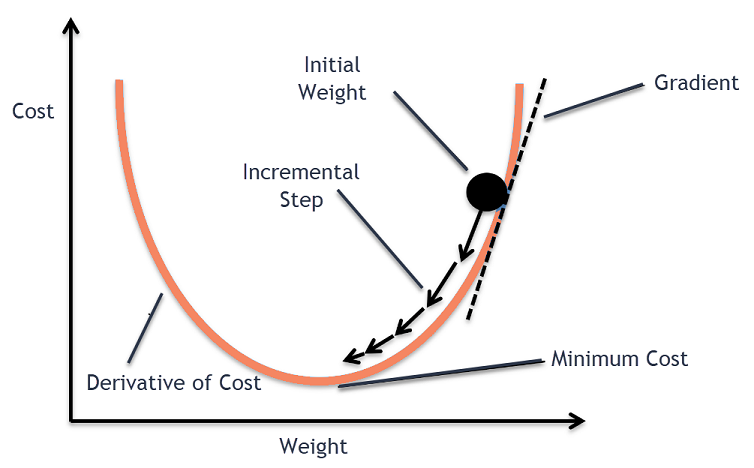
\includegraphics[width=0.6\linewidth]{ImageFiles/NeuralNetworks/graddesc}
	\caption{Gradient descent intuition \cite{GDAWML}}
	\label{fig:graddesc}
\end{figure}

Gradient descent forms the basis for various variations and extensions in optimization algorithms. These include Stochastic Gradient Descent (SGD), Mini-batch Gradient Descent, Momentum, AdaGrad, RMSprop, and Adam. These algorithms build upon the core principles of gradient descent while introducing additional mechanisms to improve convergence speed, handle non-convex loss functions, and adaptively adjust learning rates.

\subsection{Limits and problems}

ANNs have revolutionized the field of ML and have proven instrumental in tackling various challenging problems, such as image processing and recognition.

However, as with any complex model, ANNs can face the problem of overfitting. This occurs when a model becomes excessively tailored to the training data, capturing noise and irrelevant patterns. This can result in poor performance when the model is applied to new, unseen data \cite{James2013}.
Overfitting is a manifestation of the bias-variance tradeoff. In this tradeoff, models with higher complexity have the ability to fit the training data more closely (low bias), but they are also more susceptible to overfitting (high variance). Conversely, simpler models may have higher bias, potentially leading to underfitting (i.e., the model is too simplistic to capture the underlying patterns in the data).

Furthermore, alongside the overfitting issue, ANNs can also exhibit overconfidence in their predictions when providing confidence intervals \cite{9756596}. This becomes particularly concerning when these models are deployed in critical domains such as autonomous driving or the medical field.
Overconfidence means that the model is overly certain about its predictions, even when they might be incorrect. In safety-critical applications, such as autonomous driving, even a single wrong prediction by the model can have severe consequences. Similarly, in the medical field, inaccurate predictions can lead to misdiagnoses and potentially harmful treatments.